Our task is inspired by CLEVR\footnote{\url{https://cs.stanford.edu/people/jcjohns/clevr/}} \parencite{Johnson2017} and modified extensively to allow investigating the scaling behavior we aim to examine. This section will begin by describing the CLEVR stimuli and questions, explaining how we changed the images, and we created the dataset. Next, we will define the task and query format we use, and finish by will describing the two initial benchmarks we have in mind.

\begin{wrapfigure}{r}{0.5\linewidth}
\vspace{-.4in}
\begin{spacing}{1.0}
\centering
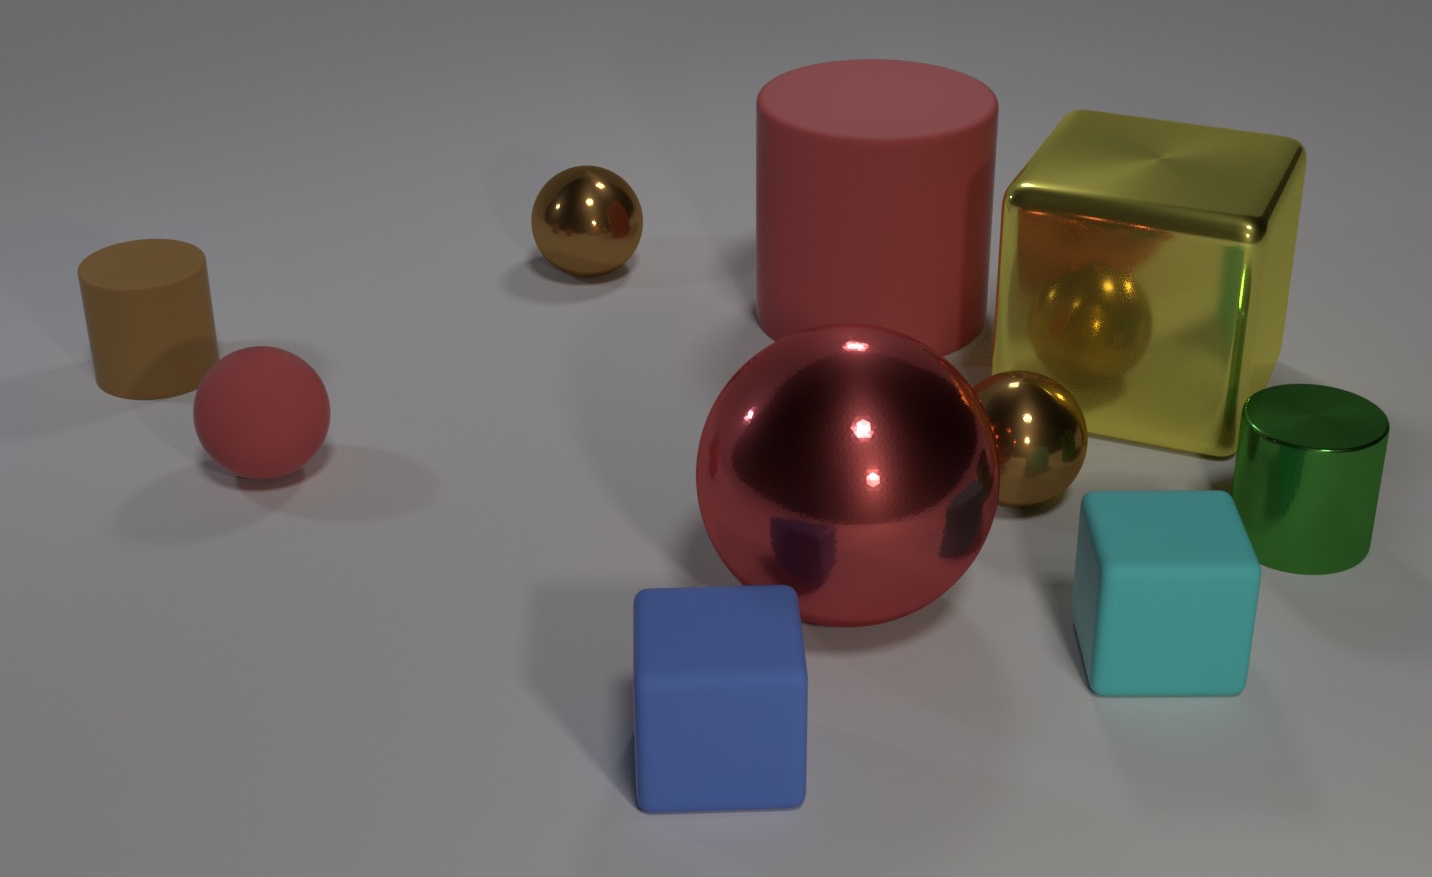
\includegraphics[width=.95\linewidth]{ch-dataset-task-benchmark/figures/dataset/original_clevr_image.png}
\caption{Original CLEVR image.}
\label{fig:dataset-clevr-image}
\end{spacing}
% \vspace{-.25in}
\end{wrapfigure}

CLEVR stands for Compositional Language and Elementary Visual Reasoning, aiming to provide researchers with synthetic (computer-generated) image dataset which allows asking different sorts of reasoning questions: comparisons, relationships, counting queries, etc. Each image in CLEVR is comprised of a number (usually 5-10) of objects, each defined by its shape (sphere, cube, or cylinder), color (one of eight options), material (metal or rubber), and size (small or large). After generating images, the CLEVR authors create queries for each image, each query an instantiation of a template filled based on the content of the image. A template such as \textit{"Do the \textless Z \textgreater \textless C \textgreater \textless M \textgreater \textless S \textgreater and the \textless Z2 \textgreater \textless C2 \textgreater \textless M2 \textgreater \textless S2 \textgreater have the same size?"} would allow asking a question such as \textit{“Do the red rubber sphere and the blue metallic sphere have the same shape?”} As these templates imply, the CLEVR database presents its queries in natural language (or as a functional program), challenging the models to reason over both textual inputs and images. Perhaps most importantly for our purposes, the authors made their entire codebase available on Github\footnote{\url{https://github.com/facebookresearch/clevr-dataset-gen/}} and did a rather reasonable job of documenting it. Their codebase uses Blender \parencite{BlenderOnlineCommunity2018}, a free and open-source 3D modeling software with a full Python API to generate the stimuli. Each stimulus is saved both as an image and as a JSON description of the scene, which allows generating valid queries and the correct answers for them. One additional source of inspiration was the Sort-of-CLEVR task introduced by \textcite{Santoro}. They provide substantially simplified visual stimuli (simple 2D drawings rather than 3D renders) and encode the questions as binary vectors, rather than natural language sentences. Sort-of-CLEVR also mixes both relational questions (\textit{``What is the shape of the object that is furthest from the gray object?’’}) and non-relational queries (\textit{``What is the shape of the gray object?’’}); the latter substantially more resembling the type of queries we decided to use.

\section{Dataset Generation}
The basic premise for our queries use is simple: we wish to train models to answer yes/no existence questions on an image. Using the original CLEVR image to the right as an example, we could query the model on \textit{``is there a purple object?''} (no), \textit{``is there a cube?''} (yes), \textit{``is there a red sphere?''} (yes), or \textit{``is there a cyan cylinder?''} (no). The CLEVR dataset is unbalanced, in that it includes eight colors, but only three types of objects (sphere, cube, and cylinder, all seen in the image above), and two materials (rubber and metal). To be able to examine the scaling behavior over the different tasks, and to avoid dataset-based biases for particular dimensions, we wanted to balance the image generation to have equal numbers of options in each dimension.

\begin{wrapfigure}{r}{0.5\linewidth}
\vspace{-.4in}
\begin{spacing}{1.0}
\centering
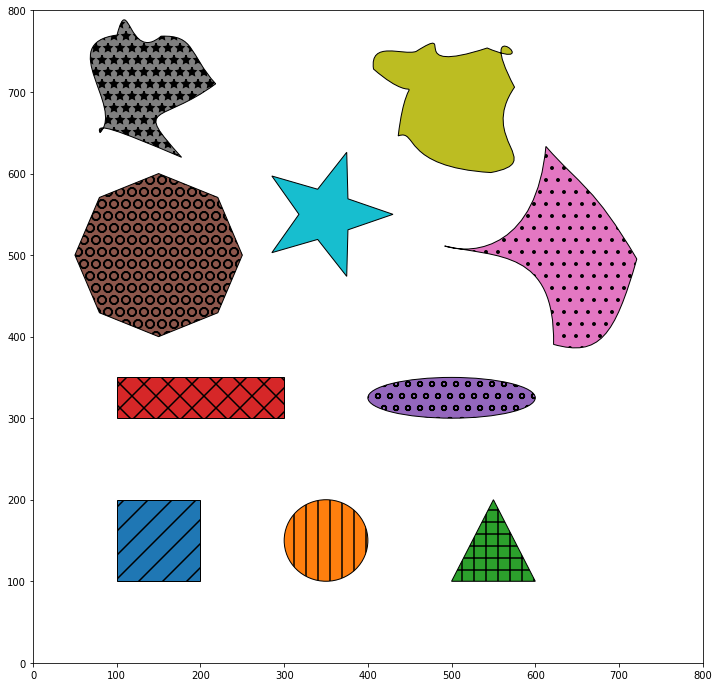
\includegraphics[width=.95\linewidth]{ch-dataset-task-benchmark/figures/dataset/matplotlib_image.png}
\caption{Matplotlib example image.}
\label{fig:dataset-matplotlib-image}
\end{spacing}
% \vspace{-.25in}
\end{wrapfigure}

We first prototyped examples using Python’s matplotlib \parencite{Hunter2007} to generate simpler stimuli (see example) but decided the results would be substantially more meaningful with a realistic visual task. We then set about adapting the codebase provided by \textcite{Johnson2017} to fit our purposes. We settled on ten colors, ten shapes, and ten materials, which provide thirty different single-property queries and three-hundred unique two-property (conjunctive) queries. 

\begin{wrapfigure}{r}{0.5\linewidth}
\vspace{-.4in}
\begin{spacing}{1.0}
\centering
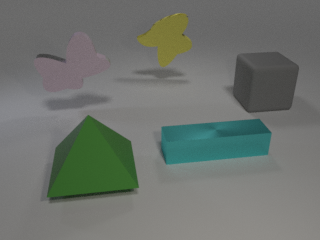
\includegraphics[width=.95\linewidth]{ch-dataset-task-benchmark/figures/dataset/first_iteration_image.png}
\caption{Example early iteration image.}
\label{fig:dataset-early-image}
\end{spacing}
% \vspace{-.25in}
\end{wrapfigure}

Choosing ten colors was easy: we picked ten reasonably equally perceptible ones\footnote{Gray, red, blue, green, brown, purple, cyan, yellow, orange, pink.} (or so we thought; we eventually discovered that our models have a hard time separating two of them). Next came the shapes: we initially created seven geometric shapes, relying on Blender’s built-in objects (such as a torus and a cone), but then realized we need additional shapes. We first experimented with different curve-enclosed shapes (in the background in the example to the right), but we were concerned with the stark difference between geometric shapes and the curved ones. After some creative thinking, we eventually settled on ten geometric shapes\footnote{Cube, sphere, cylinder, pyramid, cone, torus, rectangular box, ellipsoid, octahedron, dodecahedron}, from the mundane (cube, sphere), to elongations thereof (rectangular box, ellipsoid), to the more exotic (octahedron, dodecahedron). The materials proved the most difficult: the two in the original paper mostly differed in their reflectivity of incoming light. After following a myriad of tutorials, we realized the easiest path is to learn sufficient Blender skills to allow building image-based material textures. These allow transforming an image of a texture (e.g., bathroom tiles), alongside with maps describing the relative height at each pixel (allowing the creases between tiles to appear lower) and the reflectivity of each pixel to a Blender material definition. To apply these definitions, we also had to generate mappings from the three-dimensional surfaces of the objects to a 2D plane, on which Blender would overlay the textures; effectively, define how the objects should be cut and the surfaces laid flat. After passing through this myriad of obstacles, we were finally able to generate about fifteen textures, from which we selected ten\footnote{Metal, rubber, chainmail, marble, maze, metal weave, polka dots, rug, bathroom tiles, wooden planks.}, including the original rubber and metal, but ones as creative as a chain mail, a rug, or the previously mentioned bathroom tiles. 

\begin{wrapfigure}{r}{0.5\linewidth}
\vspace{-.2in}
\begin{spacing}{1.0}
\centering
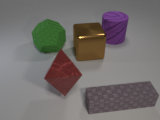
\includegraphics[width=.95\linewidth]{ch-dataset-task-benchmark/figures/dataset/final_image.png}
\caption{Example final iteration image.}
\label{fig:dataset-final-image}
\end{spacing}
% \vspace{-.25in}
\end{wrapfigure}

The image to the right is an example from the final dataset. Can you classify the shape, color, and material of each object?\footnote{Red marble octahedron, pink metallic weave rectangular box, brown metal cube, purple wooden plank cylinder, and a green chainmail dodecahedron.}

If you could tell shapes apart but had a hard time naming each color or texture, you could probably do sufficiently well, as the model is not tasked with learning the natural language mappings for these queries either. We introduce the questions to the model in binary encoding, similarly to Sort-of-CLEVR, as we wish to isolate the computer vision and meta-learning parts of the task from the natural language processing component. The query is provided as a 1x30 vector, with each block of ten units corresponding to a dimension (shape, color, and material), and each unit within a particular feature. The first unit might be mean `cube,' the twelfth `red,' and the twenty-fifth `marble.' A priori, the models will not know what feature each unit corresponds to, nor that each group of ten refer to a different dimension - but hopefully, effective meta-learning approaches will be able to extrapolate efficiently from their training, rather than pay the same cost (in training examples) for each new feature learned.  

While we made the task harder by including additional properties in each dimension, we decided to reduce a few other sources of variance, in an attempt to focus on the meta-learning. The original CLEVR dataset includes two different object sizes, while we only have one. They also include jitter, both in the orientation of the objects relative to the camera and in the precise location of the camera relative to the scene. We chose to keep both constant for now, reasoning that we could always generate a second dataset with additional visual noise should the task prove too easy. Each image we generate has four or five objects, each with a unique shape, color, and material. We settled on a size of 160x120 pixels, maintaining CLEVR’s standard 4:3 aspect ratio, but reducing each dimension by half, hopefully making the problem more computationally tractable. We also kept CLEVR’s method of assigning objects to locations in the scene randomly and checking for collisions, as it produced better results than two alternatives we examined, placing objects uniformly on a circle or in random locations on a 4x4 grid (both with some random noise to the assigned locations). The flexible nature of our implementation would allow us (or anyone else, once we make the code available on Github) to generate additional images using different parameters.

Once we settled on these final parameters for our dataset, we generated a total of fifty thousand images, split into a training set (45,000) and a test set (5000). See example images and corresponding scene descriptions (see below) here: \url{http://bit.ly/metalearning_50k_examples}. To generate these images, we used five virtual machines (VM) on Amazon Web Services (AWS). AWS offered easy access to machines with GPUs, which speed up the rendering process considerably, from about a minute per image to a few seconds, such that each VM rendered ten thousand images in just under a day. It could likely be optimized, as the object placement and collision resolution took more time (on average) than the scene rendering. We could have considered a more physically-based method, assuming each object repels other ones and simulating the dynamics between them; but the random placement proved sufficient for our purposes. We also did not attempt to explicitly balance the number of times each of the materials, colors, and shapes appear in the final dataset, and instead, we sampled them uniformly and trusted the sufficiently large sample size to overrule random fluctuations. While this worked successfully for most categories, about a month after generating the dataset we discovered some imbalances. Given 45,000 images (in the training set), four or five objects per image, and ten features within each dimension, we would expect each feature to appear, on average, in 20,250 images. The pyramid and the octahedron appear in approximately 12,000 and 14,700 samples respectively. We do not currently understand the cause, but we hypothesize that for some reason, the random placement struggled with those two shapes. If true, this underscores the need for a better placement algorithm than random assignments (or otherwise, for a better random number generator). 

Alongside each image, the script saved JSON file describing the scene. This description allowed CLEVR to parameterize their queries, knowing what sort of relational (and non-relational) queries should produce valid queries for this image. Since our queries are more straightforward than their ones, our process is equally simpler. Initial versions computed the answer for every one-dimensional query, saving a 30x30 matrix of queries (each row using a one-hot encoding), and a 30x1 vector of results (does that feature exist in the image). As this format would make designing the conjunctive queries harder, we then switched to saving a small table of object representations, which is 3x5 (dimensions x maximum number of items). In the event only four items are in the image, the last row is left empty. 

One last modification made is to provide an HDF5 file \parencite{TheHDFGroup1997} with all images and scene descriptions. Creating this file spared us from uploading fifty thousand files (or a RAR archive containing them), and was recommended in some places as an easy way to provide and package a dataset. While some recent opinions suggest against HDF5 (see \cite{Rossant2016}), we found it sufficient for our purposes, as it allows us to transfer the entire dataset in a single file.
